\section{Genetic Algorithms}

\subsection{History}

Genetic algorithms are optimisation techniques that employ the same rationale as classical Evolution as seen in nature.

Genetic Algorithms can trace their origins back to the late 1960s when they were first proposed by John Holland. Holland went on to write the first book on the subject titled \textit{Adaptation in Natural and Artificial Systems} \cite{hollandAdaptationNaturalArtificial1992a} in 1975. The field did not find much reception with Holland stating in the preface to the 1992 rerun:

\begin{displayquote}
\textit{``When this book was originally published I was very optimistic, envisioning extensive reviews and a kind of 'best seller' in the realm of monographs. Alas! That did not happen.``}
\end{displayquote}

However, in the early nineties, Genetic algorithms surged in popularity along with Artificial Intelligence as a whole leading to Holland republishing his book and solidifying his position as the field's founder.

\subsection{Definition}
In a general sense, optimisation techniques work to find the set of parameters $\mathcal{P}$ that minimise an objective function $\mathcal{F}$. 
Genetic algorithms approach this by representing these sets as individuals in a population, $P$. Over the course of multiple generations, the best solutions are determined and promoted until termination criteria are met or the maximum number of generations is reached.

As our candidates are essentially a collection of parameters to the function we are trying to optimise, we can extend our metaphor further by mapping each element of a individual to a \textit{gene} in a individual's genome. 

The representation we use in a GA is problem specific. Often we have to provide functions to facilitate the mapping between the problem specific set of possible solutions and the encoded genotype space in which we optimise. The most basic representation being a string of binary numbers.

Genetic algorithms are both \textit{probabilistically optimal} and \textit{probabilistically complete}\cite{kalaOnroadIntelligentVehicles2016} meaning that: given infinite time, not only will the algorithm find \textit{a} solution, (if one exists), it will find \textbf{the} optimal solution from the set of all possible solutions, $\mathcal{P}^*$.

\begin{algorithm}[H]
	\label{alg:GenericGA}
	\SetAlgoLined
	\KwResult{Best Solution, $p_{ \texttt{best}}$}	
	Generate initial population, $P_0$ of size $n$\;
	Evaluate fitness of each individual in $P_0$, $\{F(p_{0,1},\ldots, p_{0,n})\}$\;
	\While{termination criteria are not met}{
		\textbf{Selection}: Select individuals from $P_t$ based on their fitness\;
		\textbf{Variation}: Apply variation operators to parents from $P_t$ to produce offspring\;
		\textbf{Evaluation}: Evaluate the fitness of the newly bred individuals\;
		\textbf{Reproduction}: Generate a new population $P_{t+1}$ using individuals from $P_t$ as well as the newly bred candidates.\;
		$t$++
	}
	return $p_{\texttt{best}}$

	\caption{Modern Generic Genetic Algorithm}
\end{algorithm}

\begin{figure}[htpb]
    \centering
    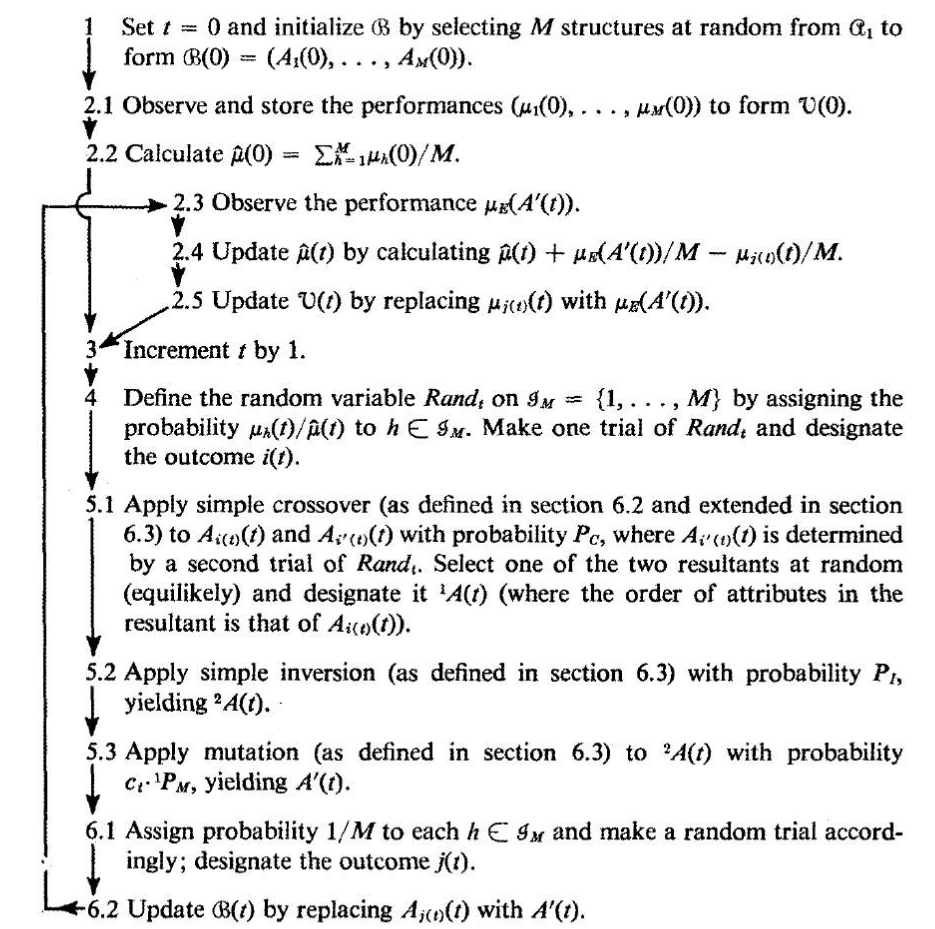
\includegraphics[width=\linewidth]{hollandAlg}
    \caption{GA algorithm outlined in Holland's Original Book\cite{hollandAdaptationNaturalArtificial1992a}}
    \label{fig:hollandAlg}
\end{figure}

As you can see from Figure \ref{fig:hollandAlg} and Algorithm \ref{alg:GenericGA} the overall shape of GAs has not changed substantially over the course of the past 50 years. Being comprised of a series of operations that a starting population is piped through until criteria are met.

\subsection{Selection}

The selection procedure 

\subsection{Variation}
\subsection{Evaluation}
\subsection{Reproduction}
\subsection{Examples}

\begin{figure}[htpb]
    \centering
    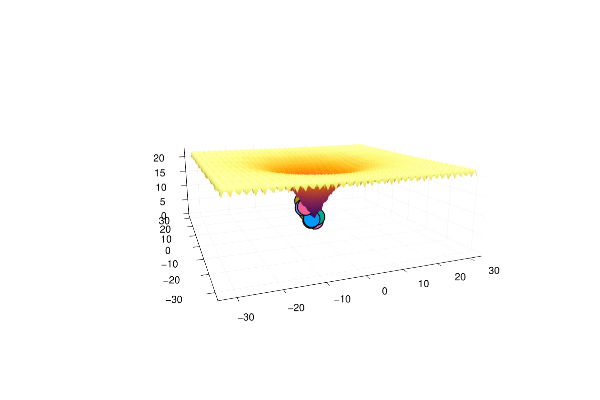
\includegraphics[width=\linewidth]{f10}
    \caption{A basic GA applied to a search space defined using the Ackley function \cite{ackleyConnectionistMachineGenetic2012} }%
    \label{fig:}
\end{figure}

\begin{figure}[htpb]
    \centering
    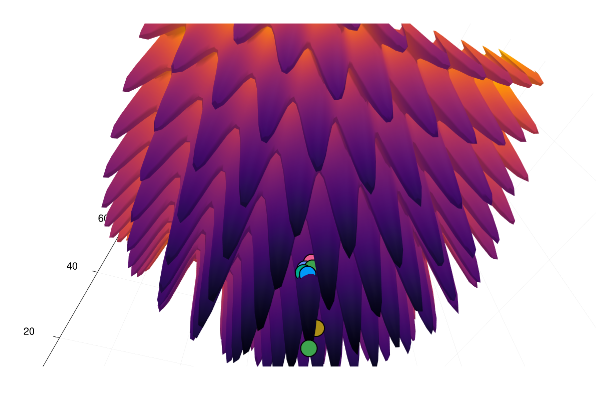
\includegraphics[width=0.8\linewidth]{rastrigin}
    \caption{A basic GA applied to a search space defined using the Rastrigin function \cite{rastriginSystemsExtremalControl1974}}%
    \label{fig:name}
\end{figure}


\section{Autonomous Road Networks}

\section{Quantum Genetic Algorithms}

\section{Alternative Technologies}
